\documentclass[11pt]{article}

\title{Before the rise of um}
\author{Timothy Gadanidis and Derek Denis}

% SIL font
\usepackage{fontspec}
\setmainfont{Charis SIL}

% margins
\usepackage[margin=1in]{geometry}

% bibliography
\RequirePackage[
    backend=biber,
    style=apa,
    sortcites=true,
sorting=nyt]
{biblatex}
\RequirePackage[american]{babel}
\bibliography{beforeum.bib}
\RequirePackage{csquotes}
\RequirePackage[american]{babel}
\DeclareLanguageMapping{american}{american-apa}

% colon postnotes
\renewcommand{\postnotedelim}{%
  \iffieldnums{postnote}
    {\addcolon~}
    {}}
\DeclareFieldFormat{postnote}{#1}
\DeclareFieldFormat{multipostnote}{#1}

% table
\usepackage{booktabs}

% figures
\usepackage{graphicx}

\usepackage[section]{placeins}

% extracts
\usepackage{newfloat}
\usepackage{caption}
\usepackage{mdframed}

\DeclareFloatingEnvironment[name=Extract]{extract}
\usepackage{dialogue}

\usepackage{linguex}

\begin{document}

\maketitle

\section{Introduction}

One of the most dramatic discourse-pragmatic changes in twentieth-century
English has progressed under the radar of laypeople and (until recently)
linguists: the rise of \emph{um} as the predominant variant of the `filled
pause' variable (UHM) at the expense of \emph{uh} \parencite{tottie2011,
fruehwald2016, wielingetal2016}.
The variation is exemplified in \Next.
\ex. \textbf{Uh} as a rule they harrowed it before they \textbf{um} drilled it.
\hfill (NIA-22)

\textcite[43]{fruehwald2016} documents this ``textbook'' change over 100+ years
of apparent time:
\emph{um} increases incrementally between generations and the rise is led by
women.
Why \emph{um}? Why did this change occur?
In this chapter, we investigate (UHM) at an early stage of change to determine
what triggered the rise of \emph{um}.
We take up the hypothesis that the rise of \emph{um} was connected to the
development of a new discourse function for the variable (UHM), that \emph{um}
came to be favoured with.
We remain agnostic about what the function is, but follow \textcite{tottie2016}
and \textcite{fruehwald2016} who suggest a correlation between utterance
position and function; and specifically \textcite[46]{fruehwald2016} who suggests
that ``turn-initial \emph{um} may be the best candidate for a new
discourse function coming into use.''
We follow essentially a variationist approach, first treating \emph{um} and
\emph{uh} as variants of a linguistic variable and using proportional analysis
to assess the role of social and linguistic factors.
We augment these results with a different quantitative perspective and examine
the relative frequency of the variable itself in discourse to help in our
interpretation.
What we find is a need to look beyond the envelope of variation, as defined, to
understand the results that we see.

\section{(UHM) as a pragmatic marker}

The exact nature of (UHM) as a linguistic feature is not a trivial question.
A great deal of ink has been spilled over whether they are produced consciously
or unconsciously, and what their purpose is.
For example, \textcite[41--42]{maclayosgood1959} characterize (UHM) as a
floor-management device which speakers insert to indicate that they do not want
to be interrupted when hesitating over what to say.
\textcite{levelt1983, levelt1989} describes (UHM) as an involuntary noise
produced as a result of production problems: ``\emph{er} apparently signals that
at the moment when trouble is detected, the source of the trouble is still
actual or quite recent. But otherwise, \emph{er} doesn't seem to mean anything.
It is a symptom, not a sign'' \parencite[484]{levelt1989}.

One problem with the involuntary ``symptom'' view is that, as
\textcite{clarkfoxtree2002} point out, speakers have some control over whether
or not they produce (UHM)---%
for example, it can be suppressed in a public speaking context (and indeed
speakers are often counselled to do so).
They argue that (UHM) is an ``interjection'' used to signify a delay, with
\emph{um} signalling longer delays than \emph{uh}.

Recently, \textcite{tottie2016} has put forward the argument that
(UHM) is a pragmatic marker that, in speech, indicates planning.
This is on the basis that (UHM) is used more frequently in contexts requiring
more speaker planning, such as narratives and responses to questions.
\textcite{tottie2017} describes (UHM) as being on a ``cline of lexicalization'',
where forms like \emph{and-uh} and \emph{but-uh} are not perceived as words, but
\emph{uh} and \emph{um} alone are.
\textcite[21--22]{tottie2017} describes the former case, where the final
consonant of a monosyllabic word such as \emph{and} or \emph{but} is immediately
followed by (UHM), as cliticized forms.
She goes on to argue that the use of (UHM) between words and silent pauses,
rather than in these cliticized forms, causes (UHM) to be perceived as a word in
the lexicon, making it available for conscious use.
If this process was a factor in (UHM)'s diachronic development, we might expect
to see an effect of cliticization at this early stage.
% TODO this is an interactional to interpersonal change

As we note above, the rise of \emph{um} has now been described extensively in
the variationist and corpus-linguistic literature, across a number of corpora
and speech communities.
The typical finding is that women have a higher \emph{um}--\emph{uh} ratio than
men, and that younger speakers have a higher \emph{um}--\emph{uh} ratio than
older ones.
This pattern has been demonstrated in various speech communities and contexts in
the United States \parencite{acton2011, fruehwald2016, wielingetal2016,
lasernaetal2014}, as well as in England and Scotland \parencite{tottie2011,
wielingetal2016}, both in real and apparent time.
\textcite{wielingetal2016} also show that this pattern extends beyond English to
five other Germanic languages: Dutch, German, Norwegian, Danish, and Faroese.

While these accounts demonstrate definitively that a change is underway, an
explanation remains elusive.
What was the trigger for this ``textbook'' change?
\textcite{fruehwald2016} and \textcite{wielingetal2016} both suggest that a new
meaning or function for \emph{um} may have emerged in English\footnote{%
    For \textcite{wielingetal2016}, this is a possible explanation for the
    crosslinguistic nature of the change: a function could have emerged in
    English and then spread through contact to the other Germanic languages.
}.
Although \textcite{fruehwald2016} found that \emph{um} and \emph{uh} appeared to
be trading frequencies, casting doubt on a functional expansion explanation, it
is possible that the emergence of a new function at some earlier point may have
played a role nearer to the beginning of the change.
Accordingly, in this chapter, we investigate data from before the rise of \emph{um} with the goal of evaluating the functional expansion hypothesis.

\section{Data and coding}

The data for this study are from the \emph{Farm Work and Farm Life Since 1890}
oral history collection \parencite{denis2016}.
The corpus consists of oral history interviews with 155 elderly farmers,
recorded in 1984.
The corpus covers five regions of Ontario, Canada: Temiskaming, Essex, Dufferin,
Niagara Region, and Eastern Ontario; for this study, speakers from the latter
two regions were considered.
Speaker birth years range from 1891 to 1919, just before \emph{um} began to take
off per \textcite{fruehwald2016}.

The interviews in each region were conducted by interviewers local to the
region: F-INT conducted the interviews in Niagara, and M-INT conducted the
interviews in Eastern Ontario.

For the purposes of this study, we follow \textcite{fruehwald2016},
\textcite{wielingetal2016}, and \textcite{tottie2016}, among others, in treating
\emph{uh} [əː] and \emph{um} [əːm] (also written as \emph{er} and \emph{erm}) as
variants of one sociolinguistic variable, termed (UHM).
It should be noted that this is not the only way that the variable context could
be defined.
For instance, \textcite{tottie2018} includes (UHM) as one element of a set
including \emph{well}, \emph{you know}, and \emph{like}, on the basis that all
of the elements are used to indicate speech planning.
In principle, \emph{unfilled} pauses, i.e., silence, could also be included in
the variable context.
However, we argue that treating \emph{um} and \emph{uh} as an individual
variable captures the two words' intuitive and structural similarity\footnote{%
    This is an (in our view justified) extension of the notion of ``structural
    equivalence'' \parencite{pichler2010, tagliamontedenis2010} to
    phonological/orthographic structure.
}, both variants being phonologically and orthographically identical, modulo
the coda.
Both variants are also single-word constructions which, unlike \emph{well},
\emph{you know}, and \emph{like}, do not appear to be derived from bleached
lexical items, but from apparently non-lexical speech sounds.
As \textcite{fruehwald2016} notes, they have also traditionally been treated as
a unique phenomenon in the psycholinguistic literature.


We extracted each instance of \emph{uh} and \emph{um} from the transcripts,
excluding unrelated instances such as \emph{uh-oh}.
Tokens from the two much-younger interviewers was also extracted, and analyzed
separately.
The transcription protocol emphasized faithful reproduction of \emph{uh} and
\emph{um}.
All interviews were carefully second-passed by the second author.

The data were coded for the following social factors:
year of birth, gender, and region (Niagara or Eastern Ontario).
Year of birth and gender were used to operationalize the change-in-progress
hypothesis.
Table~\ref{tab:speakers} presents a table of speakers by gender, region, and
year of birth.

\begin{table}[ht!]
    \centering
    \begin{tabular}{llll}
        \toprule
        ID & Gender & Region  & Year of birth \\
        \midrule
        F-INT  & F & Niagara         & unknown \\
        M-INT  & M & Eastern Ontario & unknown \\
        NIA-1   & M & Niagara         & 1906    \\
        NIA-9   & F & Niagara         & 1912    \\
        NIA-11  & M & Niagara         & 1917    \\
        NIA-12  & F & Niagara         & 1916    \\
        NIA-20  & F & Niagara         & 1911    \\
        NIA-22  & F & Niagara         & 1899    \\
        NIA-23  & M & Niagara         & 1898    \\
        NIA-24  & M & Niagara         & 1902    \\
        NIA-27  & M & Niagara         & 1911    \\
        NIA-28  & M & Niagara         & 1907    \\
        NIA-32  & F & Niagara         & 1904    \\
        NIA-35  & F & Niagara         & 1902    \\
        NIA-36  & F & Niagara         & 1903    \\
        EON-001 & M & Eastern Ontario & 1891    \\
        EON-004 & F & Eastern Ontario & 1907    \\
        EON-006 & M & Eastern Ontario & 1905    \\
        EON-012 & M & Eastern Ontario & 1910    \\
        EON-013 & F & Eastern Ontario & 1914    \\
        EON-014 & F & Eastern Ontario & 1899    \\
        EON-016 & M & Eastern Ontario & 1912    \\
        EON-019 & M & Eastern Ontario & 1904    \\
        EON-020 & F & Eastern Ontario & 1906    \\
        EON-022 & F & Eastern Ontario & 1915    \\
        EON-024 & M & Eastern Ontario & 1898    \\
        EON-028 & F & Eastern Ontario & 1919    \\
        \bottomrule
    \end{tabular}
    \caption{Table of speakers.}\label{tab:speakers}
\end{table}

We also coded for two linguistic factors.
To operationalize the functional expansion hypothesis, we coded for initial or
non-initial utterance position.
(UHM) was defined as ``initial'' if it was the first element in an utterance,
as in \Next[a], and ``non-initial'' if it was not the first element in an
utterance, as in \Next[b].
The exception was in the case of \emph{and-} or \emph{but-} cliticization, where
(UHM) was classed as ``initial'' if the containing utterance began with
\emph{and-uh} or \emph{but-uh}.
\ex.
\a.~\textbf{Um} spring time was a very busy time for everyone on the farm.
(EON-28, F/1919)
\b.~The birthdays we'd \textbf{uh}- we'd try to- we'd \textbf{uh} remember them.
(EON-001, F/1907)


To test for a potential effect of cliticization (per \citeauthor{tottie2017}'s
\citeyear{tottie2017} suggestion that this may have played a role in (UHM)'s
lexicalization) we coded each token as ``clitic'' if it occurred immediately
following \emph{and} or \emph{but}, as in \Next[a], and as ``non-clitic''
otherwise, as in \Next[b].
\ex.
\a.~If it was in school time I couldn't go unless it was Saturday
\textbf{but-uh}, auction sales were usually on Saturday. \hfill (NIA-09, F/1912)
\b.~\textbf{Um} do you know how old you were when you started? \hfill (F-INT)

\section{Results}

\subsection{Proportional frequency}

Table~\ref{t:comparison} shows how our data compare with previous communities
analyzed.
The first block summarizes our data from Niagara and Eastern Ontario, as well as
F-INT and M-INT, the two younger interviewers.
The second block summarizes results from previous work on the Switchboard corpus
\parencite{switchboard}, the Fisher corpus \parencite{fisher}, the Philadelphia
Neighborhood Corpus (PNC) \parencite{labovrosenfelder2011}, and the British
National Corpus (BNC) (\citeyear{bnc}).
The numbers for all of these other corpora are drawn from
\textcite{wielingetal2016}.

\begin{table}[ht!]
    \centering
    \begin{tabular}{lrrrrrr}
        \toprule
                    & Raw N       & Raw N       & \%          & Mean              & Mean             & Mean     \\
        Community   & \textit{uh} & \textit{um} & \textit{um} & \textit{uh} /1000 & \textit{um}/1000 & UHM/1000 \\
        \midrule
        Niagara     & 1864        & 357         & 16.1        & 21.3              & 4.1              & 25.4     \\
        E. Ont.     & 1563        & 168         & 9.7         & 22.6              & 2.4              & 25.0     \\
        F-INT       & 321         & 318         & 49.8        & 12.4              & 12.3             & 24.7     \\
        M-INT       & 255         & 51          & 16.7        & 13.2              & 2.6              & 15.8     \\
        \midrule
        Switchboard & ---         & ---         & 28.3        & 22.1              & 7.5              & 29.6     \\
        Fisher      & ---         & ---         & 64.1        & 6.8               & 9.9              & 16.7     \\
        PNC         & ---         & ---         & 27.6        & 13.2              & 4.5              & 17.7     \\
        BNC         & ---         & ---         & 46.1        & 4.5               & 4.3              & 8.8      \\
        \bottomrule
    \end{tabular}
    \caption{Cross-community comparison}
    \label{t:comparison}
\end{table}

% TODO: describe how to read the tables and charts

As can be seen in the table, \emph{um} is less frequent in our data compared to
the more recent corpora; the female interviewer uses it around half the time,
while the male interviewer's rate is comparable to the farmers'.
Relative frequency of (UHM) taken as a whole is on par with other corpora, but
we are cautious about making such a comparison because each corpus was collected
and transcribed differently \parencite[for related discussion,
see][]{pichler2010}.

Looking at individual speakers' rates, we can see that all speakers use both
\emph{uh} and \emph{um}, but there is no clear pattern by age
(Figure~\ref{fig:indivage}) or gender (Figure~\ref{fig:indivgender}).

% TODO: these figures probably need to be remade in black and white
%       plus there are a lot of visual improvements that could be made

\begin{figure}[htpb]
    \centering
    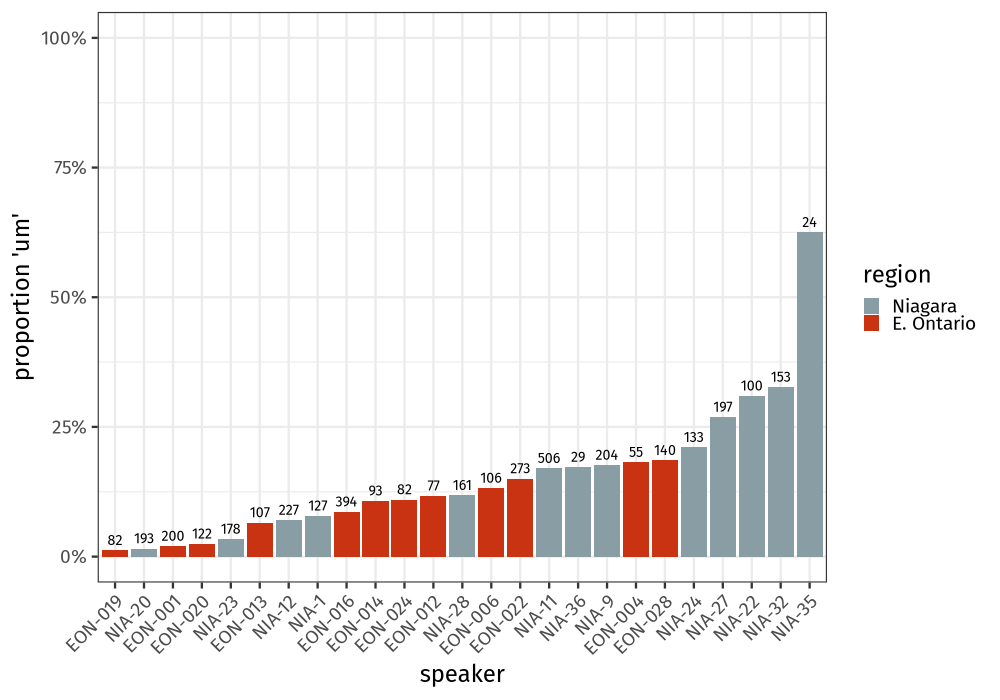
\includegraphics[width=0.8\linewidth]{figures/indivage.png}
    \caption{Proportion \emph{um} per speaker by age.}
    \label{fig:indivage}
\end{figure}

\begin{figure}[htpb]
    \centering
    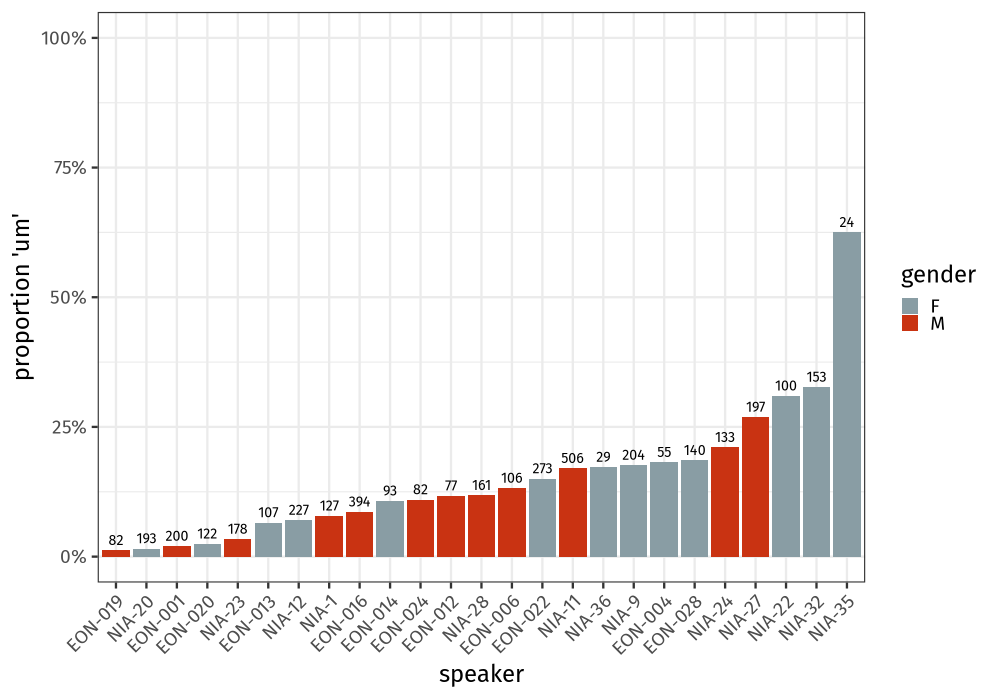
\includegraphics[width=0.8\linewidth]{figures/indivgender.png}
    \caption{Proportion \emph{um} per speaker by gender.}
    \label{fig:indivgender}
\end{figure}

Figure~\ref{fig:apparenttime} shows the proportion of \emph{um} in apparent
time.
In the plot to the left, year of birth is binned into five-year increments,
whereas in the plot to the right, year of birth is continuous.
In both cases, there is a modest trend upward over time.
To determine the possible predictors underlying this trend, in the following
figures we split the data by gender, position and cliticization.
Figure~\ref{fig:apparentgender} shows the pattern when splitting speakers by
gender.
Starting around 1905, women use \emph{um} slightly less often than men do, with
both genders' \emph{um} rates trending slightly upward over time.
Figure~\ref{fig:apparentposition} shows the pattern when splitting tokens by
position (initial vs.\ non-initial).
Starting around 1905, \emph{um} is used more frequently in initial position than
in non-initial position.
Figure~\ref{fig:apparentclitic} shows the pattern when splitting tokens by
cliticization with \emph{and} or \emph{but} and position.
\emph{Um}'s proportional increase appears to be limited to non-cliticized
initial tokens.

\begin{figure}[htpb]
    \centering
    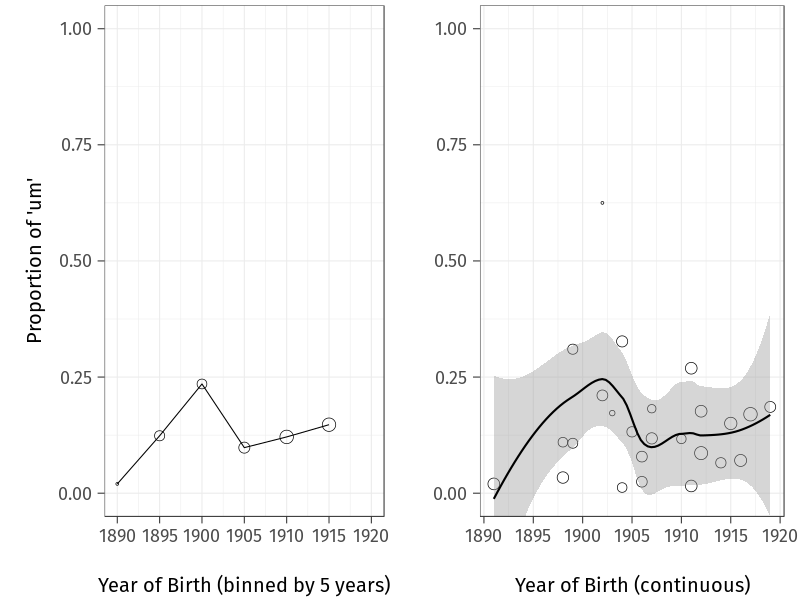
\includegraphics[width=0.8\linewidth]{figures/apparenttime.png}
    \caption{Proportion \emph{um} in apparent time.}
    \label{fig:apparenttime}
\end{figure}

\begin{figure}[htpb]
    \centering
    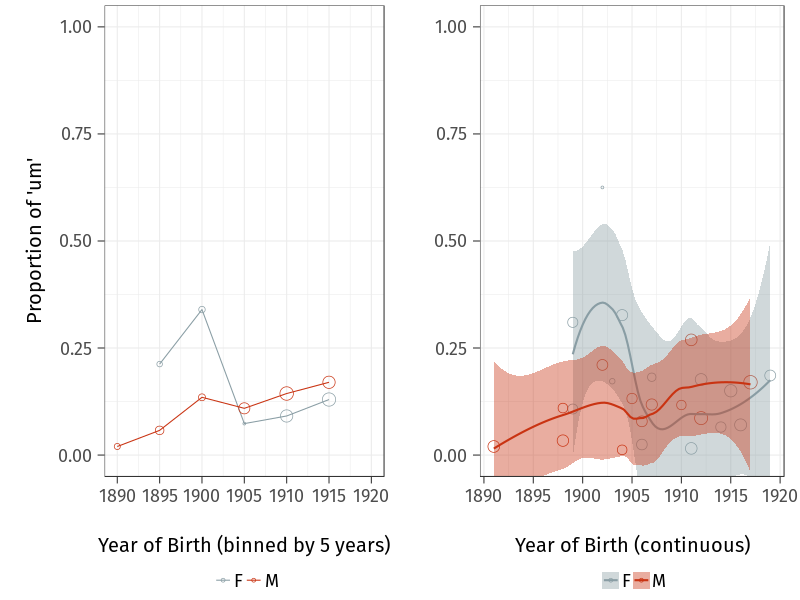
\includegraphics[width=0.8\linewidth]{figures/apparentgender.png}
    \caption{Proportion \emph{um} in apparent time, by gender.}
    \label{fig:apparentgender}
\end{figure}

\begin{figure}[htpb]
    \centering
    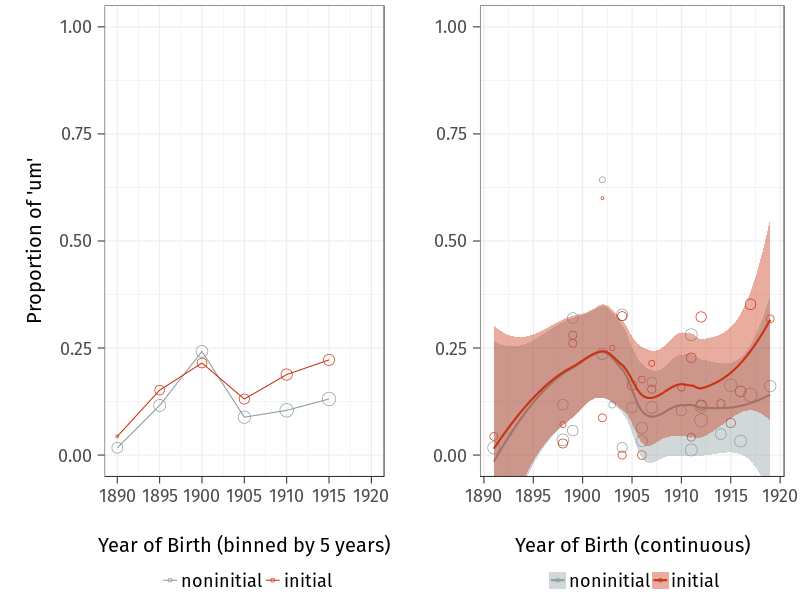
\includegraphics[width=0.8\linewidth]{figures/apparentposition.png}
    \caption{Proportion \emph{um} in apparent time, by position.}
    \label{fig:apparentposition}
\end{figure}

\begin{figure}[htpb]
    \centering
    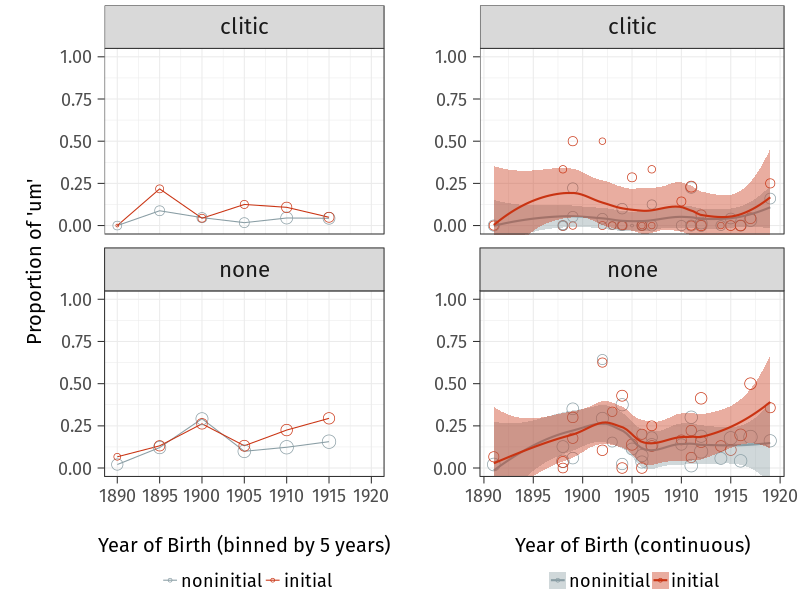
\includegraphics[width=0.8\linewidth]{figures/apparentclitic.png}
    \caption{Proportion \emph{um} in apparent time, by position and
    cliticization.}
    \label{fig:apparentclitic}
\end{figure}

Figure~\ref{fig:farmertree} shows a conditional inference tree for all farmers.
Conditional inference trees are statistical models built by repeatedly splitting
the data based on a set of covariates, using a significance test procedure to
select the variables to split by.
The model in Figure~\ref{fig:farmertree} contained the predictors position
(``pos''), cliticization (``clitic''), gender (which was not selected for any
splits), and year of birth.
The model confirms several of the patterns indicated in
Figures~\ref{fig:apparenttime}--\ref{fig:apparentclitic}.
The tree splits first at cliticization, with cliticized (UHM) having a low
overall \emph{um} rate.
Within the cliticized tokens, there is a slight difference between noninitial
and initial (UHM), with initial tokens having a higher \emph{um} rate (9.39\%)
than noninitial ones (4.35\%).
Within the noncliticized tokens, there is an effect of year of birth:
speakers born after 1898 have a much higher \emph{um} rate in noncliticized
tokens than that of speakers born in 1898 or earlier (4.65\%).
This is especially true in initial position:
noninitial cliticized tokens have a lower \emph{um} rate (16.10\%) than initial
ones (21.90\%).

\begin{figure}[htpb]
    \centering
    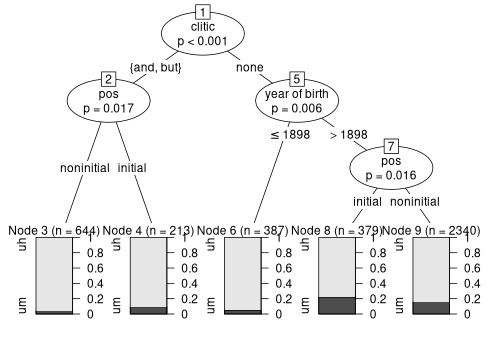
\includegraphics[width=0.8\linewidth]{figures/ctreefarmers.png}
    \caption{Conditional inference tree for farmers.}
    \label{fig:farmertree}
\end{figure}

Figure~\ref{fig:interviewertree} shows a conditional inference tree for the two
interviewers.
The model contained position and cliticization (the interviewers' years of birth
are not known, and there are only two speakers in any case).
As shown in the tree, the internal constraints are much the same, but the
baseline \emph{um} rate is much higher (due in large part to the female
interviewer).
\emph{Um} is the least common in the cliticized forms (13.90\%).
In non-cliticized forms, there is a split by position, where initial tokens
favour \emph{um} (53.20\%) compared to non-initial tokens (40.90\%).

\begin{figure}[htpb]
    \centering
    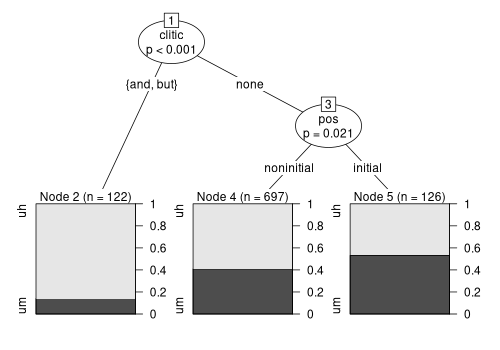
\includegraphics[width=0.8\linewidth]{figures/ctreeinterviewers.png}
    \caption{Conditional inference tree for interviewers.}
    \label{fig:interviewertree}
\end{figure}

Taken together, the results presented in this section appear to show the
beginning of the change toward \emph{um} that has been observed by other
researchers.
While other work has shown that women lead this change, in our data, older women
actually use more \emph{um} than the younger women.
% TODO: no gender effect.
% connect this to Tagliamonte and D'Arcy (2007?)
% frequency and variation in the community
% labov 2001

Looking at internal factors, we can see that cliticized forms, like
\emph{and-uh}, favour \emph{uh}.
There is some evidence for positional divergence, possibly consistent with a new
utterance-initial discourse function that favours \emph{um}
\parencite[cf.][, who found no turn-positional difference]{fruehwald2016}.
Conditional inference trees confirm that the internal constraints persist with
the younger speakers, while their baseline \emph{um} rate is higher.

% TODO: functional expansion teaser

\subsection{Relative frequency}

\textcite{fruehwald2016} tests the hypothesis that functional expansion
triggered the rise of um by considering changes to the relative frequency of
variants over time (e.g., frequency of \emph{um} or \emph{uh} per 1000 words).
When a new discourse-pragmatic function emerges, we expect that these functions
would add to the relative frequency of the feature; it is being used overall
more frequently because it appears additionally in a new context.
If the new function is restricted to one variant, the relative frequency of that
variant should rise, with little change to the relative frequency of the other
variant.
In other words, we expect a fishtail pattern as with the lexical frequency of
\emph{computer} and \emph{typewriter} over time: once \emph{computer} gained its
contemporary meaning, its relative frequency took off as that meaning became
more frequent.
This is illustrated in Figure~\ref{fig:fishtail} \parencite[Figure 3
from][]{fruehwald2016}: looking at the proportion of \emph{computer} over
\emph{typewriter} (left graph), \emph{computer} appears to replace
\emph{typewriter} over time; but looking at the relative frequency of each word
(right graph), it's clear that \emph{typewriter} remained stable as
\emph{computer} took off, being used in contexts that \emph{typewriter} had
never been used before.

\begin{figure}[htpb]
    \centering
    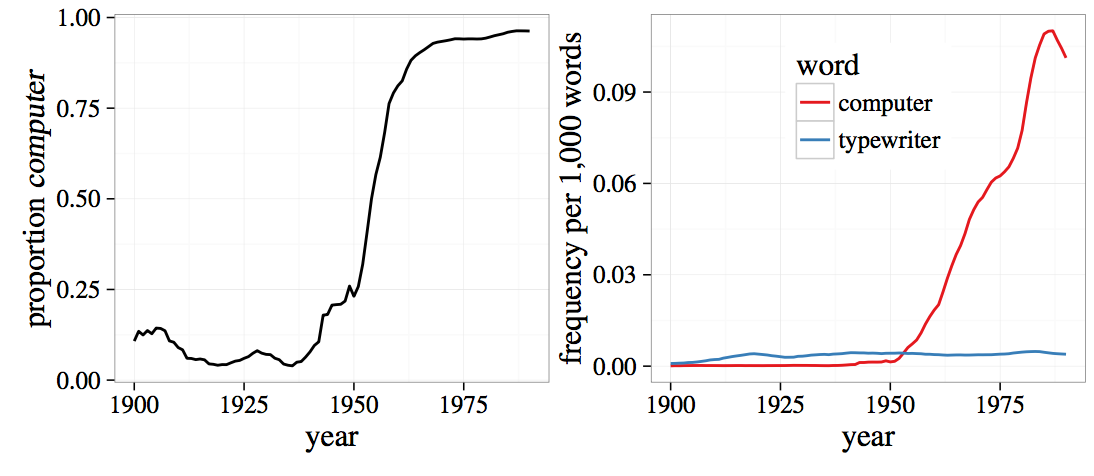
\includegraphics[width=0.8\linewidth]{figures/fishtail.png}
    \caption{Proportional frequency and relative frequency of \emph{computer}
    and \emph{typewriter} \parencite[Figure 3 from][]{fruehwald2016}.}
    \label{fig:fishtail}
\end{figure}

If a new discourse function is what led to the rise of \emph{um}, we should
expect to see a similar fishtail pattern, with \emph{um} rising and \emph{uh}
remaining stable.
Conversely, if \emph{um} were straightforwardly replacing \emph{uh}, we should
expect \emph{uh} to fall concurrently with \emph{um}'s rise.

Figure~\ref{fig:relfreq} shows the frequency of \emph{um} and \emph{uh} per 1000
words for each of the farmers.
There is some evidence of a fishtail pattern, but in the opposite direction as
expected: \emph{uh} is increasing as \emph{um} remains relatively stable.
The pattern is more extreme when we split the data by position, as in
Figure~\ref{fig:relfreqposition}.
In initial position, both \emph{um} and \emph{uh} are largely stable, whereas in
noninitial position, \emph{uh} alone is increasing.
Splitting the data again by gender, we can see that the increase can be
attributed to the female speakers---%
there is no apparent increase over apparent time for male speakers,
but the older female speakers have a relatively lower \emph{uh} rate, rising to
match the male speakers by the 1910s.

\begin{figure}[htpb]
    \centering
    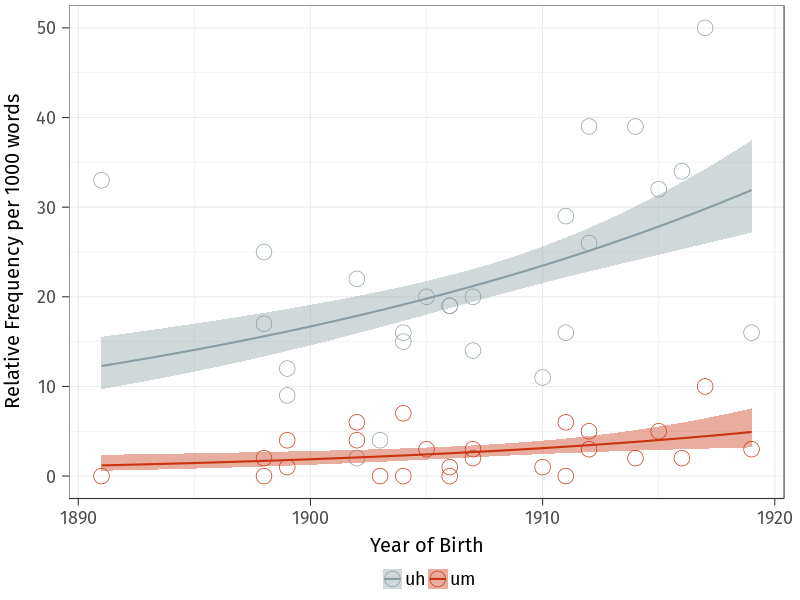
\includegraphics[width=0.8\linewidth]{figures/relfreq.png}
    \caption{Frequency of \emph{uh} and \emph{um} per 1000 words}%
    \label{fig:relfreq}
\end{figure}

\begin{figure}[htpb]
    \centering
    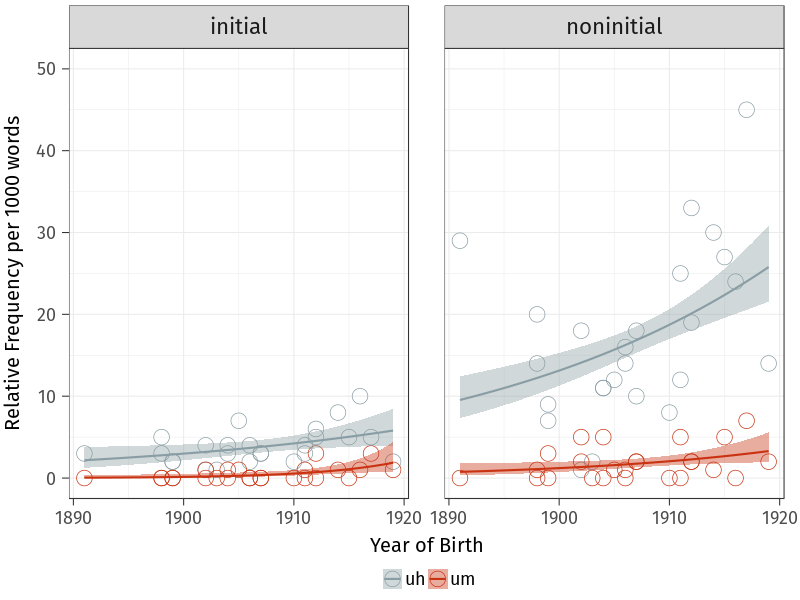
\includegraphics[width=0.8\linewidth]{figures/relfreqposition.png}
    \caption{Frequency of \emph{uh} and \emph{um} per 1000 words, by position}%
    \label{fig:relfreqposition}
\end{figure}

\begin{figure}[htpb]
    \centering
    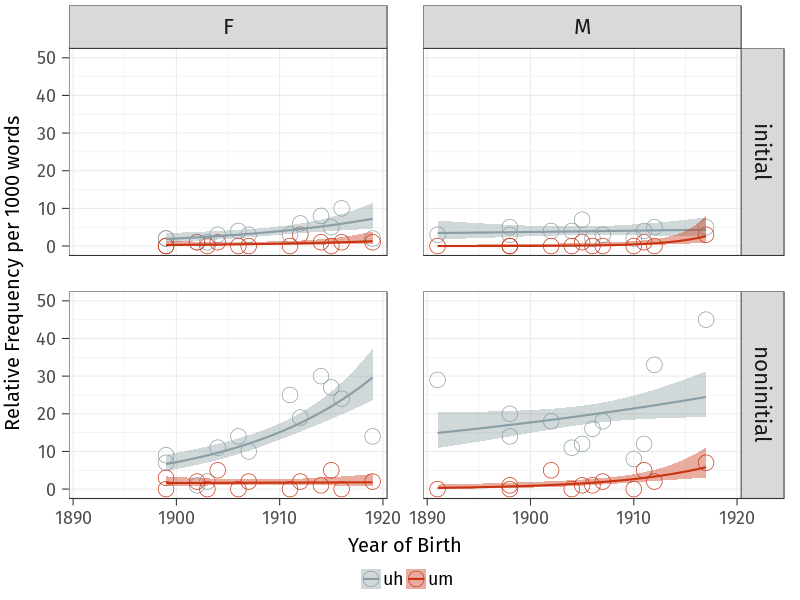
\includegraphics[width=0.8\linewidth]{figures/relfreqgenderposition.png}
    \caption{Frequency of \emph{uh} and \emph{um} per 1000 words, by position
    and gender}%
    \label{fig:relfreqgenderposition}
\end{figure}

% TODO: poisson model

\section{Discussion}

Exploring data from before the rise of \emph{um} has not yielded a definitive
explanation for the change.
Looking at the proportional frequency, we do find that for the younger
farmers,
\emph{um} appears more frequent than \emph{uh} in initial position, and the same
is the case for the two (much younger) interviewers.
Alone, this could be taken as suggestive evidence in favour of a new,
initial-position function for \emph{um}.
Looking at the relative frequency, however, we see that the pattern does not
appear to be driven by an increase of \emph{um} in initial position---%
like \textcite{fruehwald2016}, we do not find strong evidence that a new,
utterance-initial function for \emph{um} is behind the rise of \emph{um}.
The question as to what the trigger for the rise of \emph{um} was remains.
However, we find evidence of a different change:
younger speakers fill more pauses than their older counterparts, and when they
do, they are largely using uncliticized \emph{uh} in non-initial position.

This difference is illustrated by Extracts~\ref{ext:highuhm}
and~\ref{ext:lowuhm}:
two passages of about the same length from NIA-11, a younger woman (born 1917),
and NIA-36, an older woman (born 1903).
In the transcriptions, (UHM) is bolded, and unfilled pauses are indicated using
(.) or (\ldots), depending on the length of the pause.
In her extract, NIA-11 uses (UHM) eight times---%
all but one of which are \emph{uh}.
In sharp contrast, NIA-36 does not use (UHM) once, opting instead for lengthy,
unfilled pauses.
With respect to (UHM), the two speakers employ fundamentally different discourse
strategies.

While our data are too early to shed much light on the rise of \emph{um}, and it
is important to be careful when generalizing across corpora and speech
communities, it is possible that the \emph{uh}-led shift from unfilled to filled
pauses played a role in the competition between \emph{um} and \emph{uh} in the
years to come.
For example, if \emph{uh} became specialized to non-initial
position, which often appears to indicate word-search \parencite{tottie2016,
tottie2017}, it may have become a less desirable variant (frequent word-search
possibly giving the impression of disfluency).
That word-search function may previously have been associated with unfilled
pauses.
% TODO fully lay out the argument from Tottie 2017
% pauses in extract 2 seem to happen right before she's recalling information
% same places where extract 1 UH appears
% pull in examples from Tottie
% pausing to recall information --- similar to wordsearch
However, we have to stress that more work would be needed for us to be able to
go beyond this kind of speculation.

\begin{extract}[ht!]
    \begin{mdframed}[leftmargin=10pt,rightmargin=10pt]
        \begin{dialogue}

            \speak{INT} And what types of fruit (.) did you grow?

            \speak{NIA-11} Well the \textbf{uh} (.) originally \textbf{uh} when they
            came- \textbf{uh} grandfather bought the property in nineteen hundred
            and \textbf{uh} (.) \textbf{um} (.) to begin with there was very- there
            were very few fruit trees on it and they planted (.) \textbf{uh} (.) our
            orchard of \textbf{uh} (.)  peaches. And \textbf{uh} waiting- while they
            waited for the peaches to come into bearing, they planted raspberries
            between the rows, so it started out as principally a raspberry farm I
            suppose but (.) it evolved into a farm that \textbf{uh} principally grew
            peaches and cherries, mainly sweet~cherries.
        \end{dialogue}
    \end{mdframed}
    \caption{High (UHM) user}\label{ext:highuhm}
\end{extract}

\begin{extract}[ht!]
    \begin{mdframed}[leftmargin=10pt,rightmargin=10pt]
        \begin{dialogue}

            \speak{INT} Okay. And how much (.) older was the very oldest?

            \speak{NIA-36} The oldest was born (\ldots) in eighteen ninety two
            (\ldots) and then my sister Lianne, eighteen ninety four (\ldots)
            Greg, eighteen ninety eight (.) Sally nineteen hundred and one
            (\ldots) I was born nineteen hundred and three (.) and that's it.

            \speak{INT} Okay, and how old was your dad when you were born? At-

            \speak{NIA-36} (\ldots) I- (\ldots) how old was my dad when I was born? Oh.

            \speak{INT} I think we had figured out that he was probably
            somewhere around forty five.

            \speak{NIA-36} Oh yes.

            \speak{INT} And your mom was?

            \speak{NIA-36} Thirty (.) five?

            \speak{INT} Thirty- oh-

            \speak{NIA-36} Is that it?

            \speak{INT} Yup. Good.

        \end{dialogue}
    \end{mdframed}
    \caption{Low (UHM) user}\label{ext:lowuhm}
\end{extract}

These results highlight the importance of viewing discourse-pragmatic variation
from multiple angles:
the two perspectives we employ here, a proportional analysis and a relative
frequency analysis, provide complementary information about the functional
expansion hypothesis.
Considering only the proportional data might suggest that a new function for
\emph{um} is emerging, but that's not the full story.
Studies of discourse-pragmatic variation require both of these perspectives.
% TODO cite thompson and mulac 1991
% just looking at the proportions, you see stability over time.
% looking at frequency of use of EPs in general changed, one position not the
% other.

\printbibliography

\end{document}
